\section{Introdução}

Este projeto tem como objetivo a criação de um \textit{device driver} para a
plataforma Linux e um vírus específico para este \textit{driver}, além de 
realizar estudo sobre os dois temas.

\subsection{\textit{Device Driver}}

Um \textit{device driver} é um mecanismo especial do Linux kernel que permite
ao programador construir uma lógica através de uma interface de comunicação
com um dispositivo de IO (\textit{Input and Output}). Com essa interface
o \textit{driver} pode ser construído a parte do resto do kernel e "plugado" em tempo
real quando necessário.

Na construção de um \textit{device driver}, é importante esclarecer dois conceitos:
\begin{itemize}
  \item \textit{\textbf{Kernel Space}}: o kernel gerencia o \textit{hardware} de maneira simples, oferecendo
    ao usuário um simples e uniforme modo de programação, as interfaces. Sendo assim,
    o kernel promove uma ponte entre o usuário/programador e o \textit{hardware}. Qualquer
    subrotina e função que façam parte do kernel são considerados parte do \textit{kernel space}.

  \item \textit{\textbf{User Space}}: os programas \textit{end-user} como o UNIX shell ou outra aplicação GUI são
    parte do \textit{user space}. Elas se comunicam com o \textit{hardware} do sistema, mas não diretamente.
    O kernel promove funções de suporte para essas aplicações e o próprio kernel realiza
    a gerência do \textit{hardware}.

\end{itemize}

Em resumo, kernel oferece subrotinas ou funções para as aplicações \textit{end-user} para interagir
com o \textit{hardware} (user space), mas também oferece funções para a comunicação baixo nível do sistema
com o \textit{hardware} (kernel space).

\subsubsection{USB Driver}

Em um sistema operacional Linux, um dispositivo USB sempre será detectado quando inserido.
A detecção em nível de \textit{hardware} é feito pela controladora de USB - \textit{USB Host Controller}. A controladora
correspondênte irá enviar as informações da camada \textit{low-level} para a camada \textit{higher-level} que contém
as especificações do protocolo USB. As especificações de protocolo transformam as infomações recebidas
sobre o dispositivo e os propaga para a camada de USB genérica - \textit{USB Core} - definida no espaço
do kernel. Nesse ponto, o device é detectado mesmo sem haver um \textit{driver} associado específicamente a ele.

\begin{figure}[H]
  \centering
  \caption{Camadas do sistema USB Linux}
  \label{fig:usblinux}
  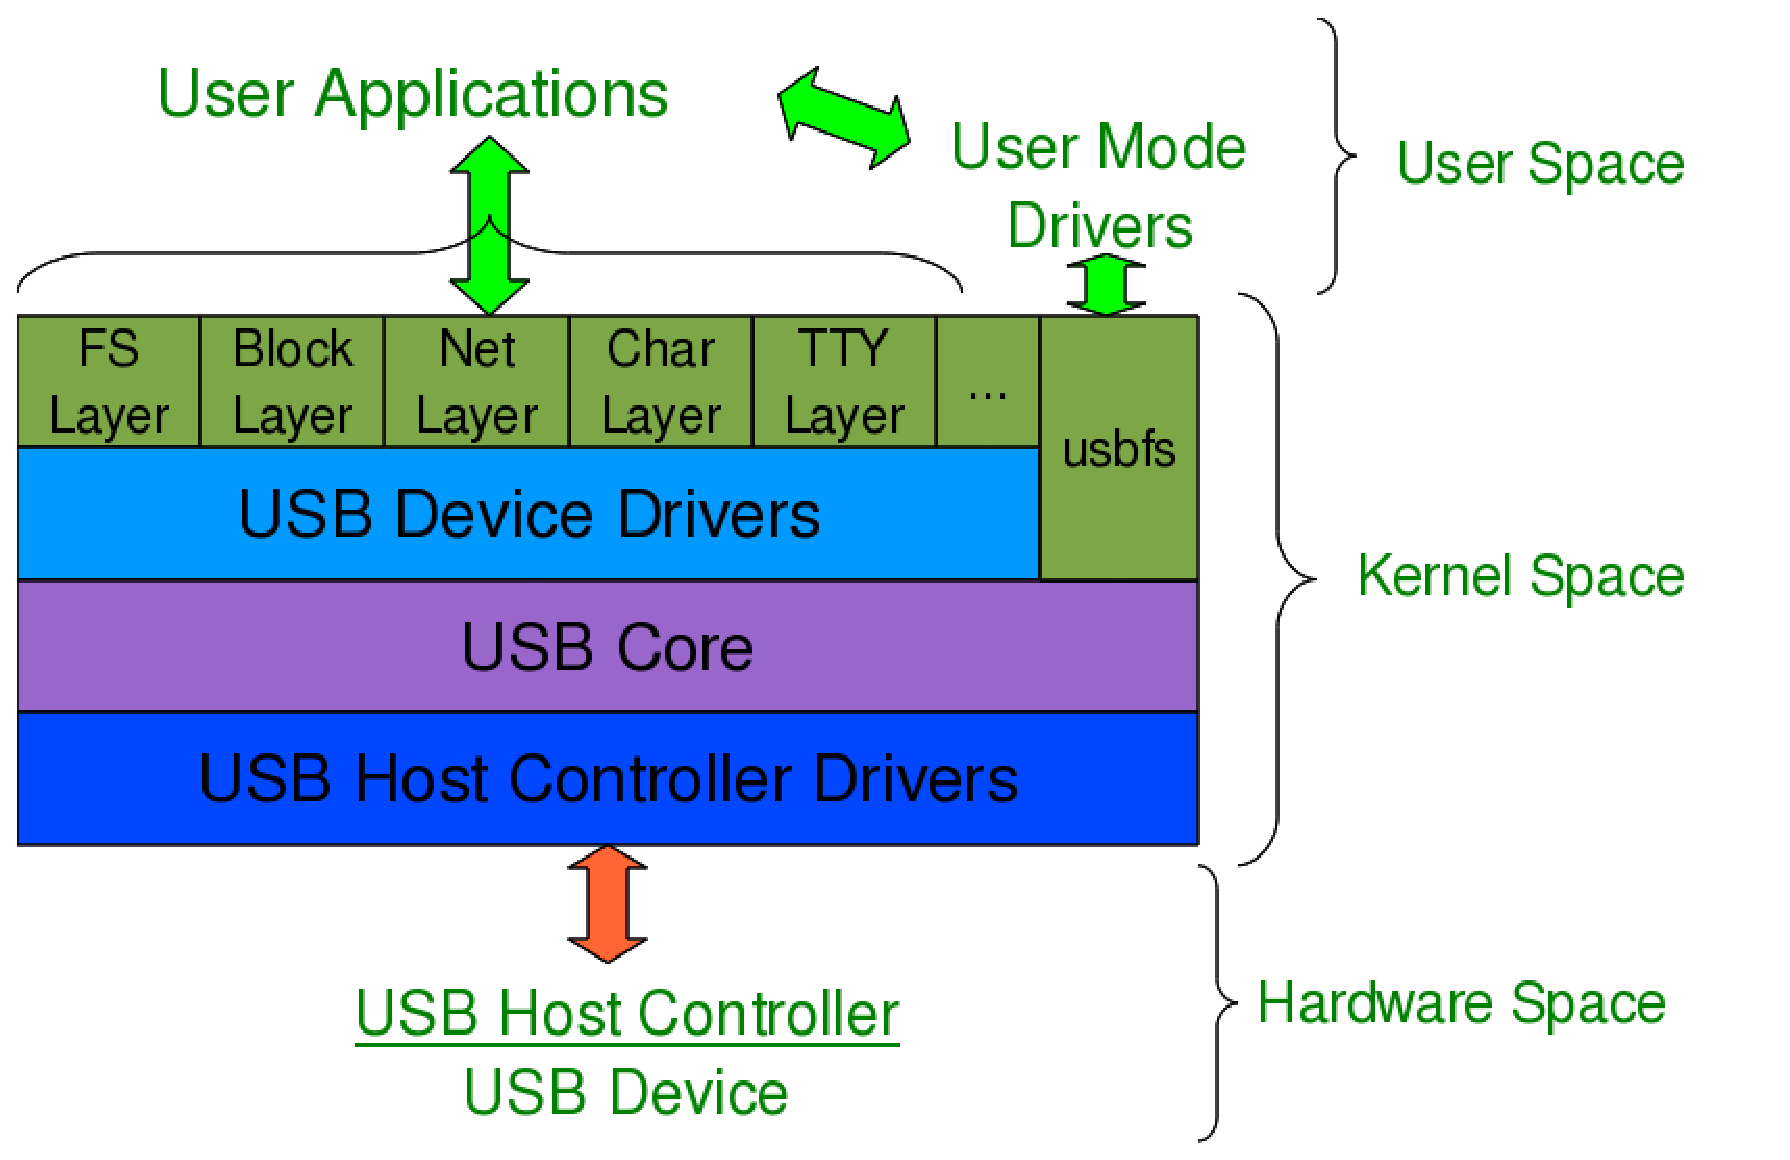
\includegraphics[width=0.9\textwidth]{figure/usbgeral.eps}
\end{figure}

A camada de USB core se comunica com o dispositivo utilizando os \textit{urb} que é descrito com uma estrutura
(\textit{struct urb}). Os urbs são utilizado para enviar e receber dados de um USB endpoint de um
dispositivo específico. O ciclo de vida de um urb é basicamente:
\begin{enumerate}
  \item Criado por um driver;
  \item Associado a um endpoint de um dispositivo USB;
  \item Submetido para o USB code pelo driver;
  \item Submetido para o USB host controller específico do dispositivo;
  \item Processado pelo USB host controller que transfere para o dispositivo;
  \item Quando o urb é completado, o USB host controller notifica o driver.
\end{enumerate}

Um urb é criado dinamicamente e  pode ser concelado a qualquer momento pelo driver ou pelo USB core
se o dispositivo for removido do sistema.

Um dispositívo válido de USB tem uma estrutura composta por: \textit{configurations, interface e endpoints}.
\begin{itemize}
  \item \textbf{Configurations}: é o perfil do dispositivo. É usado pelo USB Core para inicializar o dispositivo;
  \item \textbf{Interface}: corresponde a funcionalidade do dispositívo;
  \item \textbf{Endpoint}: são como \textit{pipes} que transferem informações para o dispositívo ou para o computador.
\end{itemize}

O ambiente Linux suporta apenas uma \textit{configuration} por dispositivo. Para cada \textit{configuration}, o dispositivo
pode tem uma ou mais \textit{interface}. Como dito, uma \textit{interface} representa uma funcionalidade do dispositivo,
por exemplo, uma impressora multifuncional tem as funções de imprimir, scanner e fax. Portanto, um
dispositivo USB, ao contrário de outros dispositivos, é associado por \textit{interface} ao invés do dispositivo
como um todo. Em resumo, um dispositivo USB pode tem vários drivers e várias \textit{interfaces} podem ter o
mesmo driver. E para cada \textit{interface} tem-se vários \textit{endpoints}. A figura \ref{fig:usbdevice} mostra essa
estrutura.

\begin{figure}[H]
  \centering
  \caption{Estrutura de um dispositivo.}
  \label{fig:usbdevice}
  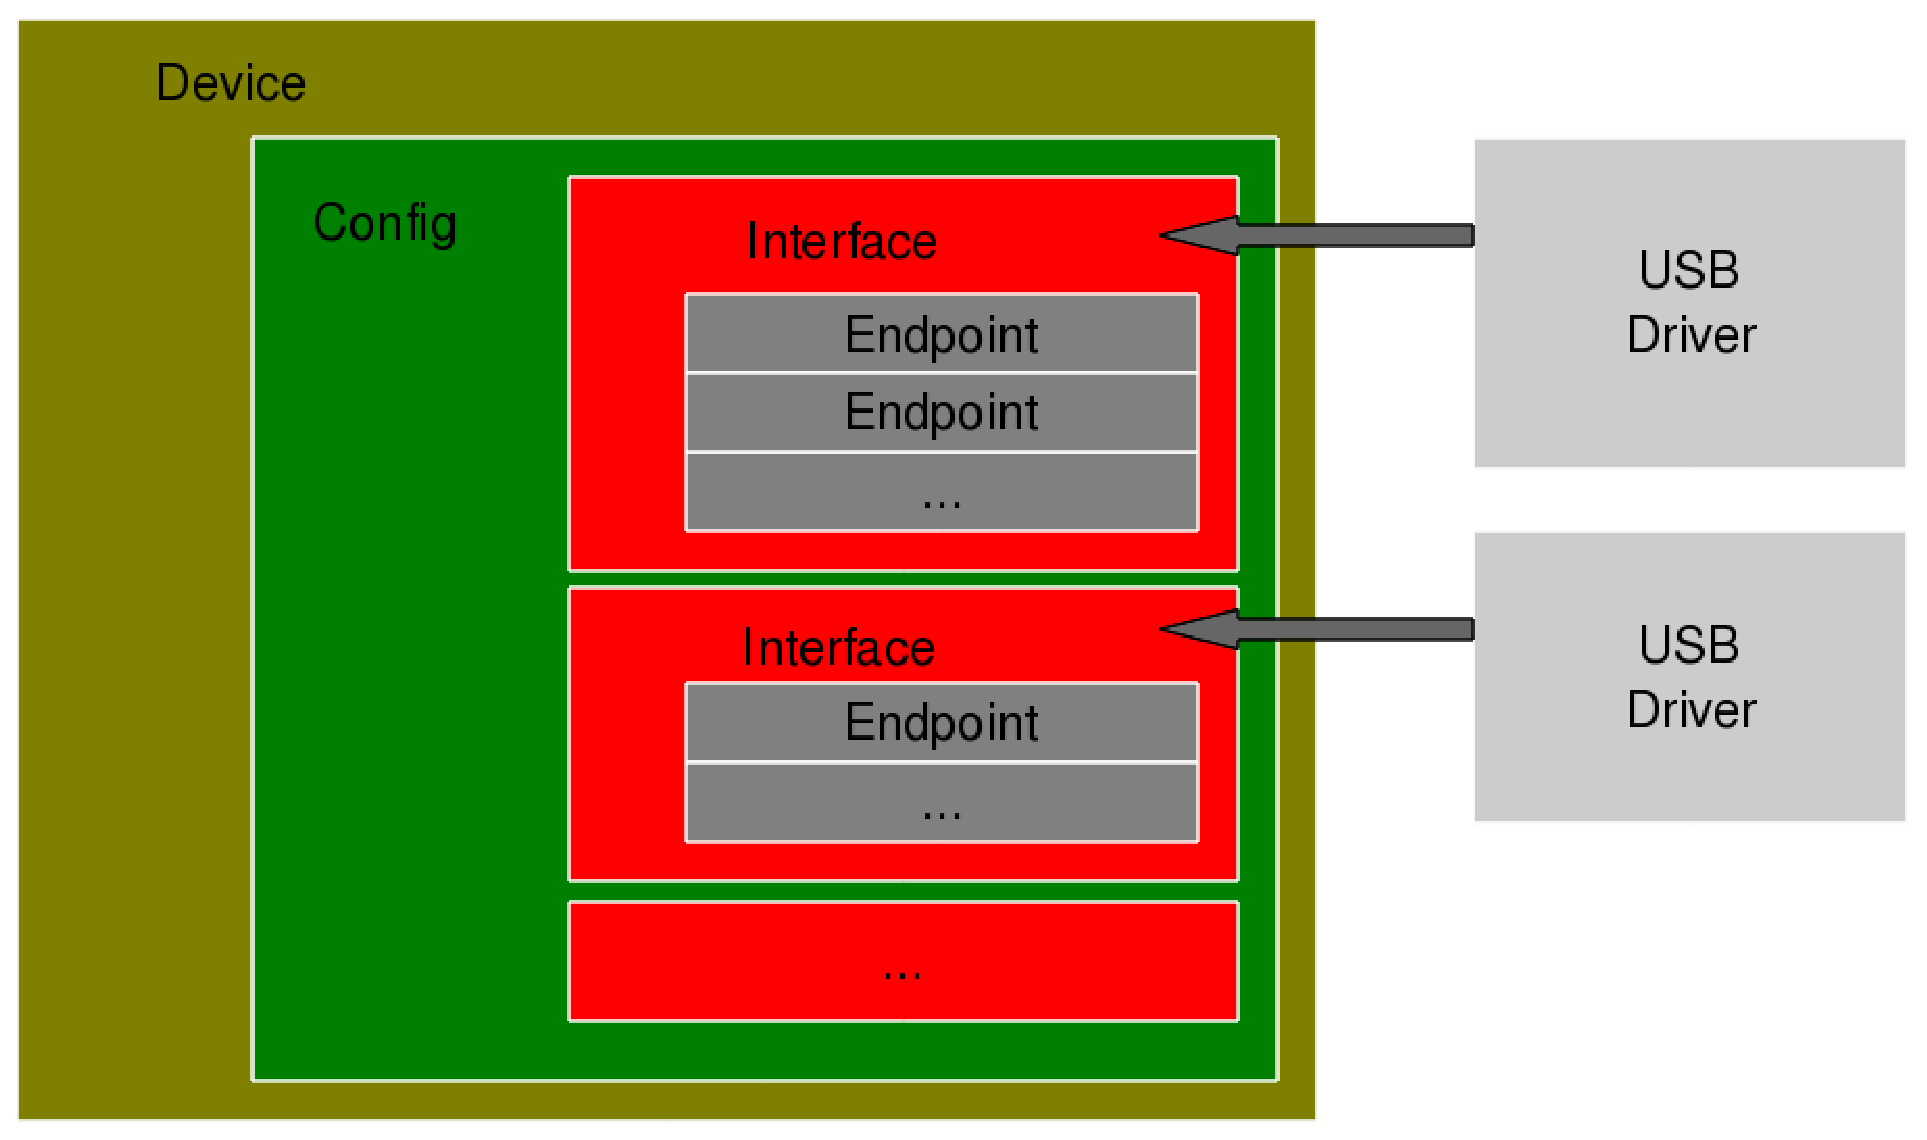
\includegraphics[width=0.9\textwidth]{figure/usbdevice.eps}
\end{figure}

Na seção \ref{utils} será mostrado algumas aplicações e comandos que são utilizados para identificar
as informações de um dispositivo USB.



\subsection{Vírus}

\begin{itemize}
  \item \textbf{Vírus de \textit{Boot}}: o vírus de boot foi um dos primeiros vírus a surgirem no mundo,
    ele foi criado com o objetivo de danificar o setor de inicialização do disco rígido,
    no qual a sua forma de propagação era através de um disquete contaminado. O vírus se
    alojava no primeiro setor do disco flexível e ocupava cerca de 1k ou menos em um
    disquete que era de 360k mais ou menos. Na inicialização do boot com o disquete
    contaminado, o vírus se aloja na memória no endereço 0000:7C00h da bios e começa
    a se auto-executar , prejudicando assim a inicialização do computador

  \item \textbf{Vírus de Macro}: o vírus macro encontrado-se frequentemente em documentos ou é
    inserido em códigos maliciosos em programas de processamento de texto, podendo ter
    origem em docs anexados ou em e-mails, no qual o vírus pode ser transferido para o
    computador depois de clicar em ligações de “phishing” ou mesmo em propagandas. Esses
    vírus são difíceis de serem identificados e o seu maior risco é que tem uma grande
    capacidade de se propagar, no qual eles podem causar danificações nos documentos infectados.
\end{itemize}

\section{Descrição do Problema}

Dentro do contexto de \textit{device drivers}, existe o aspecto de segurança do sistema operacional.
Ataques externos são considerados qualquer tentativa de recuperar dados sigilosos, danificar
o sistema em sí ou utilizar recursos computacionais para realizar outras operações não autorizadas.
Com visão deste cenário, será necessário construír um vírus para um \textit{driver} específico.
No caso deste projeto, o vírus será direcionado para um \textit{driver} construído especificamente para
este objetivo, contendo dois comportamentos: normal e anormal, para apresentar o
funcionamento do vírus.

\section{Metodologia}

O grupo adotou reuniões presenciais e remotas para desenvolvimento do trabalho. A partir
disso algumas ferramentas foram utilizadas para que se pudesse desenvolver o trabalho em
equipe. As ferramentas foram:

\begin{itemize}
  \item Google hangout;
  \item Tmate;
  \item Github;
\end{itemize}

O Google hangout fora utilizado em conjunto com o tmate para provimento de reuniões remotas
e compartilhamento do terminal respectivamente. O tmate com seu compartilhamento de terminal
via ssh permite todos integrantes tenham acesso á um terminal único em tempo real. Desse modo,
o pareamento remoto torna-se facilitado. O Github é utilizado como ferramento de versionamento
de código. 

\section{\textit{Checklist} de Requisitos}

A lista abaixo contem os requisitos espeficicados para o laboratório e o
seu status de implementação da solução proposta.

\begin{itemize}
  \item (  ) Estudo sobre Vírus: tipos de vírus e vermes, como eles se disseminam;
  \item (OK) Estudo sobre \textit{Device Drivers}: funcionamento e como construir;
  \item (OK) Tutorial da construção do \textit{Device Drivers} (Anexo A);
  \item (  ) Propor um \textit{Device Drive} com duas forma de funcionamento: normal e anormal;
  \item (OK) O \textit{Device Drive} deve ser gerenciado por lsmdo, insmod, rmmod;
  \item (OK) O \textit{Device Drive} deve apresentar na tela o que está ocorrendo;
  \item (OK) Usar processos em ambiente Linux/Linguagem C;
  \item (  ) Executar o programa várias vezes e criar um quadro adequado para apresetar os resultados;
\end{itemize}

\section{Descrição da Solução}

A solução proposta consta com a leitura de um device driver para um mouse USB.

\subsection{Comandos de Suporte}
\label{util}
Durante a construção de um \textit{device driver} existem algumas aplicações e comandos que facilitam
a obtenção de informações sobre o dispositivo e o \textit{driver}.

%TODO: adicionar os comandos de
% lsusb
%   lsusb -vd vendorID:prodID
% lsmod
% insmod
% rmmod
% cat /proc/kallsyms

% wireshark

\subsection{Funções da API}



\section{Conclusão}
%TODO: opniões sobre o projetom
%   Dificuldades
%   Lições aprendidas

%TODO: Anexo contendo:
%   Descrição sobre as funções de manipulação de devices drivers: estrutura de dados e exemplos
%   Apresentar outra estrutura da soloção implementada

%TODO: Anexo contendo:
%   Descrição sobre tipos de virus: virus de setor de boot e virus de macro
%   Alternativas de proteção
